\chapter{Magyarázatgenerálás}\label{ch:exp}
%Diverse feature visualizations reveal invariances in early layers of  deep neural networks
%https://arxiv.org/abs/1807.10589v1
%Feature Visualization
%https://distill.pub/2017/feature-visualization/
%What Uncertainties Do We Need in Bayesian Deep Learning for Computer Vision?
%https://arxiv.org/pdf/1703.04977.pdf

A modern rendszerekben a tesztelésre nagy hangsúlyt fordítanak, főleg ha biztonságkritikus rendszerekről van szó. A neurális hálózatok és a gépi tanulás területe tesztelhetőség szempontjából jelentősen le van maradva a klasszikus megoldásokkal szemben. Míg egy konvencionális program esetében használhatók egység, modul, integrációs tesztek és még sok más, a használt algoritmusok helyessége általában bizonyított és bár kimerítő tesztelés legtöbbször nem lehetséges, de a a működésre általában korlátok adhatóak. Ezzel szemben, alap esetben egy neurális háló esetén csak a konkrét bemenetekre adott választ tudjuk vizsgálni, ez több szinten is problémás. A tesztre használható példák száma limitált, többet előállítani belőlük költséges, vagy zárt határidőn belül potenciálisan lehetetlen is. A meglévő példáknak is csak egy kis hányadát használhatjuk tesztelésre, mivel szét kell őket osztani tanító,validációs és teszt halmazokra. Mindez azt eredményezi, hogy a bemenetek teljes állapotterének nagyon elenyésző hányadát tudjuk csak tesztelni. Ezen kívül zajosak lehetnek a példák, azaz bizonyos tulajdonságok, amik a valóságban sokkal kevésbé, vagy egyáltalán nem korrelálnak a célváltozóval, a véletlen folytán nagy korrelációt mutatnak az a rendelkezésre álló adathalmazban. Például képek osztályozásánál az kategorizálandó objektumokat ábrázoló képekben a háttérnek valami sajátossága van amit nem vettünk figyelembe, esetleg egy bizonyos kategóriába tartozó képek azonos napszakban, azonos éghajlaton, vagy más karakterisztikájú kamerával lettek felvéve, mint a többi példa. Ekkor a hálózat lehet hogy nem a vizsgálandó objektum, hanem annak háttere alapján kategorizálja be a képeket. Többek közt az ilyen zajok felfedezésére használható a magyarázat generálás.

\section{Általánosságban}
%TODO megnézni hogy a bevezetőben ezt hogy írtam.

A magyarázat generálási módszerek két fő kategóriába sorolhatóak, képeket feldolgozó hálózatok esetén alkalmazott a tulajdonság vizualizáció módszere és az általánosan alkalmazható hozzátulajdonítás módszere (angolul \foreignlanguage{english}{attribution}). 

\subsection{Tulajdonság vizualizáció}

Legfőképpen a mély neurális hálózatoknál alkalmazott gradiens módszerekre alapuló magyarázat generálási típus. Alap koncepciója hogy egy már valamilyen célra betanított hálózatra vagy annak egy bizonyos részére meghatároz egy hibafüggvényt, majd a bemenetet úgy módosítja, hogy a kimenet hibája csökkenjen. Tulajdonképpen egy hibavisszaterjesztés algoritmust használva nem a súlyok, hanem a bemeneti értékek parciális deriváltjait határozza meg.

\begin{figure}[H]
    \centering
    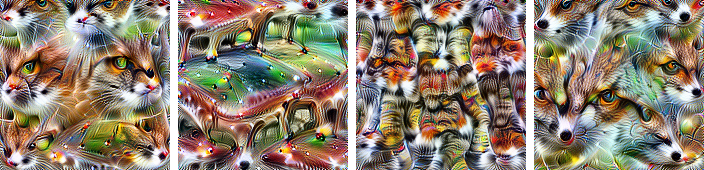
\includegraphics[width=\linewidth]{figures/feature_visualization.png}
    \caption{GoogleNet hálózat 4e inception moduljának egy vizualizációja}
    \label{fig:featurevisualization}
\end{figure}

A hibafüggvény általában arra optimalizál, hogy minél magasabb értéket vegyen fel egy neuron vagy réteg kimenete, ezáltal olyan képet létrehozva amit "érdekesnek talál" a háló.

A kiinduló állapotként gyakran alkalmaznak véletlen bemenetet és tanító példákat is. A tanító példákra valid kritika, hogy nem lehet tudni az eredmény milyen mértékben a háló belső karakterisztikája és milyen mértékben csak a bemenet egy torzítása. Másik probléma, hogy egy kép nem reprezentatív a háló működésére, mert nem csak arra a mintára vagyunk kíváncsiak amire leginkább aktiválódik a vizsgált hálózatrész, hanem azokra is amikre kevésbé reagál, de még fontosnak találja őket. Erre a problémára nem megoldás több véletlen állapotból indítani az optimalizációt, mivel gyakran nagyon hasonló eredmények alakulnak ki. 

A hiba függvény olyan módú változtatása, hogy penalizálja a korábbiakhoz hasonló képeket javít a képek sokszínűségén, de a képek közti különbség számolásnak is vannak korlátai (például azonos minták jelenléte felcserélve nagy távolságot eredményez), ezért így sem lehet konzisztensen előállítani az összes lényeges mintát.

A tulajdonság vizualizáció segít intuíció szerzésében a hálók belső működésével kapcsolatban, ez nagyon értékes mivel a mélyebb megértés segíti a kutatókat. Ezen kívül vizuálisan és érdekesek, ami közelebb hozhatja az embereket a gépi tanuláshoz. Viszont a bevezetőben felvázolt célra nem a legmegfelelőbbek. Ennek oka, hogy maguk az eredmények nehezen értelmezhetőek, ezért ha még tartalmaznak is utalást egy problémára a tanításban, az nehezen lesz megfogható. Továbbá ezek a módszerek nagyrészt specifikusak a háló implementációjára (kivéve ha a kimenetet tekintjük, de annak is megvannak a saját problémái), ezért általános alkalmazásuk nehézkes. Ezen okokból bár ezen a területen is sok érdekes algoritmus létezik, nem tartoznak szorosan ezen dokumentum tematikájához.

\section{Hozzátulajdonítás (attribution)}

Ezen módszer kimenetekhez bemeneti tulajdonságokat tulajdonít, ezáltal mutatva, hogy mely bemenetek fontosak a feldolgozásban. Tulajdonképpen megmagyarázza, hogy egy bemenetnél mire alapozta döntését a modell.






\section{Potenciális előnyök}